\chapter{Introduction}

\section{Motivation}
In an immersive virtual reality environment, an avatar is more than just a digital representation of its user. It serves as a virtual persona and a gateway to social interaction with one another as well as to one's sense of presence in the virtual world \Citep{Kyrlitsias.2022}. By infusing an avatar with personalized touches, individuals can amplify their sense of identity and immerse themselves more deeply in virtual environments, fostering a stronger connection between their physical and digital selves \Citep{Seo.2017,Canales.2024}. Through stylization, users not only express their individuality but also enhance their presence in virtual spaces, creating a more meaningful and immersive experience \Citep{Nguyen-Phuoc.2023,Dubosc.2021}.

Formally, an avatar is a type of virtual human (VH) that represents a user in a virtual world. An avatar is perceivable by the user and/or by other users in multiuser virtual environments \citep{Nowak.2018}. To create a personalized avatar, one must first generate a 3D model of the user. This can be done using a 3D scanner or 3D modeling software. Once the 3D model is created, it can be stylized in various ways to create a unique and personalized avatar. For an avatar to be appealing, recognizable, and truly embody the user, it must retain key features while undergoing partial stylization.

\begin{figure}[ht]
	\centering
	\begin{subfigure}{0.40\linewidth}
		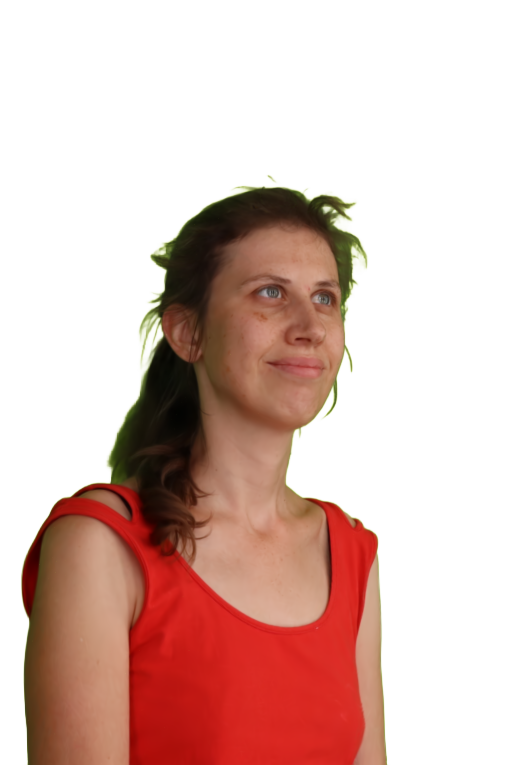
\includegraphics[width=0.45\linewidth]{Figures/results/initials/dora/12_render.png}
		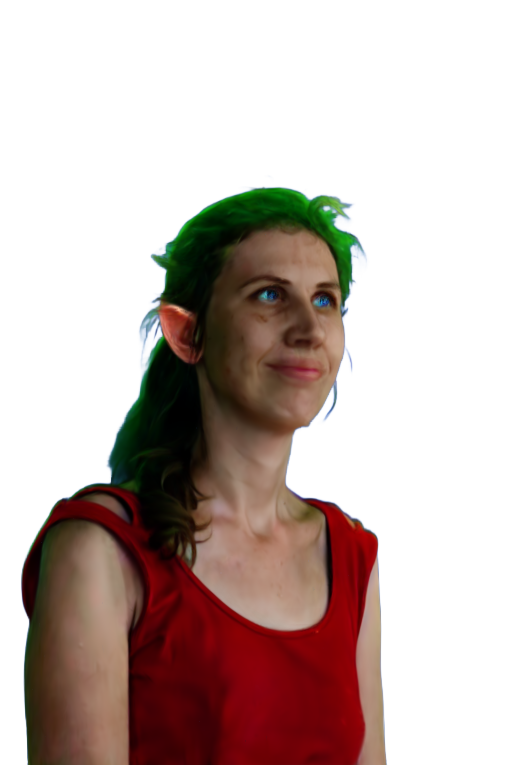
\includegraphics[width=0.45\linewidth]{Figures/results/low/dora_elf/12_render.png}
		\caption{"Make her look like a Tolkien elf"}
	\end{subfigure}
	\begin{subfigure}{0.40\linewidth}
		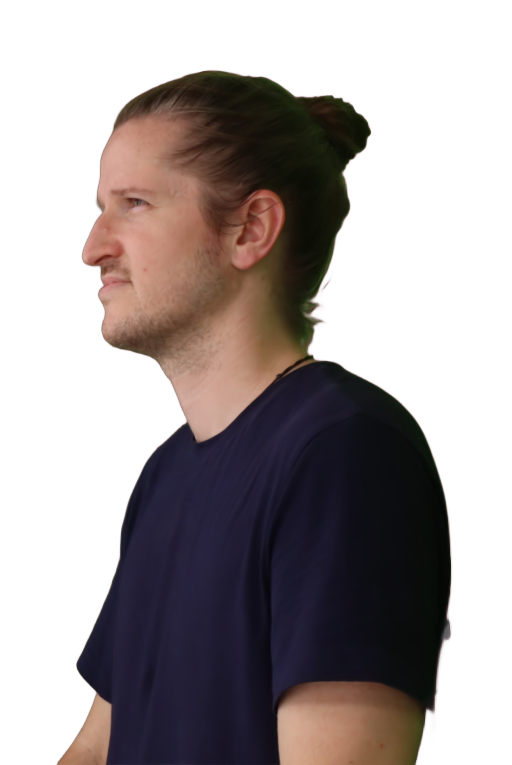
\includegraphics[width=0.45\linewidth]{Figures/results/initials/ephra/26_render.png}
		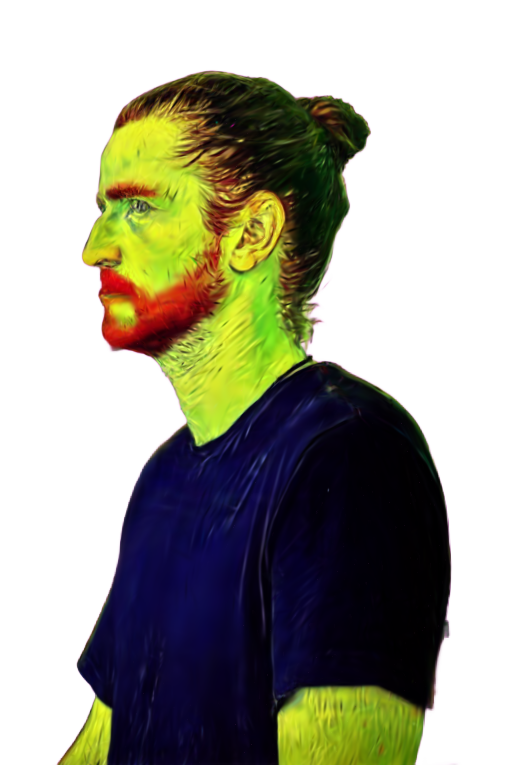
\includegraphics[width=0.45\linewidth]{Figures/results/high/ephra_vangogh/26_render.png}
		\caption{"As if a painting in Van Gogh style"}
	\end{subfigure}
	\begin{subfigure}{0.40\linewidth}
		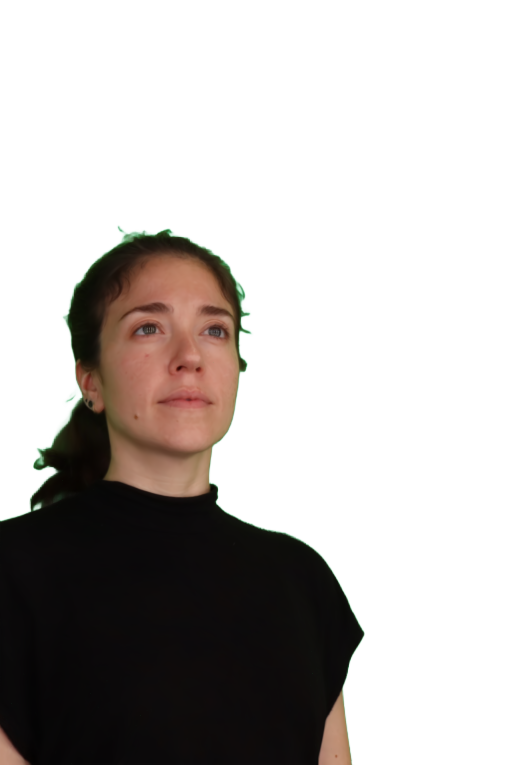
\includegraphics[width=0.45\linewidth]{Figures/results/initials/irene/11_render.png}
		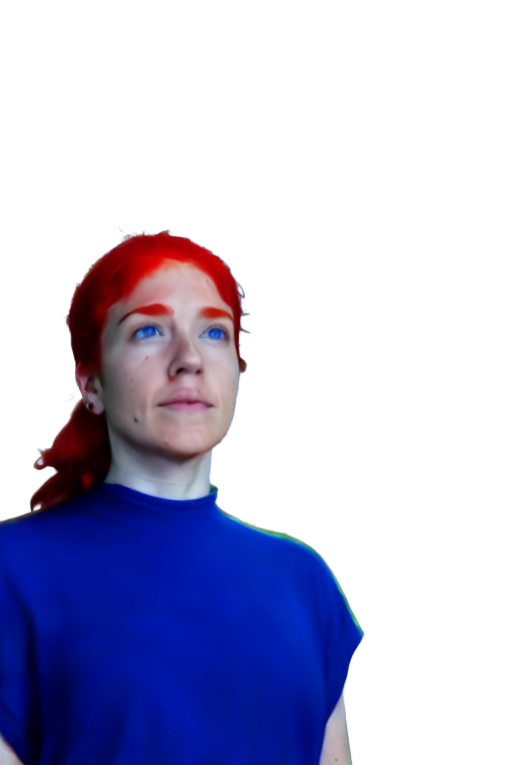
\includegraphics[width=0.45\linewidth]{Figures/results/high/irene_red/11_render.png}
		\caption{"Give her red hair and blue shirt"}
	\end{subfigure}
	\begin{subfigure}{0.40\linewidth}
		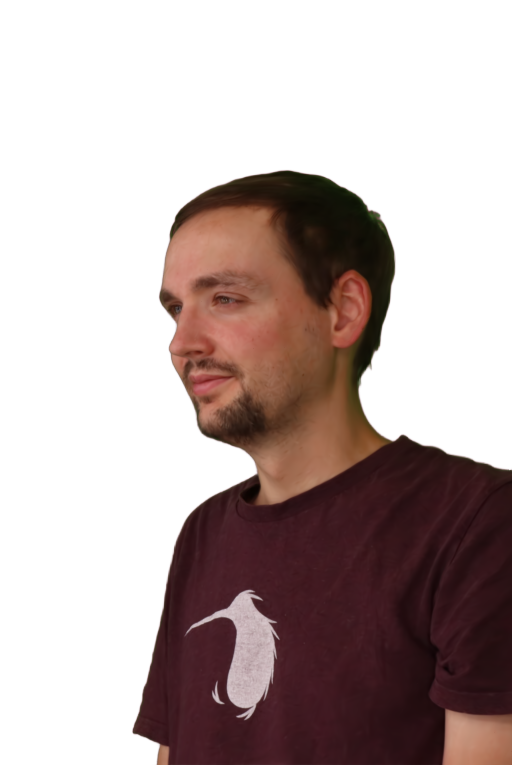
\includegraphics[width=0.45\linewidth]{Figures/results/initials/simon/27_render.png}
		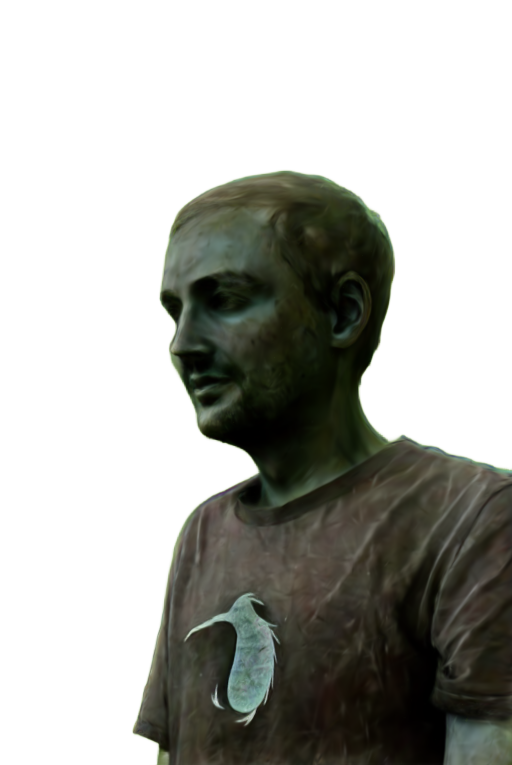
\includegraphics[width=0.45\linewidth]{Figures/results/high/simon_stone/27_render.png}
		\caption{"Turn him into a stone statue"}
	\end{subfigure}
	\caption{The left image shows the original avatar, while the right image shows the stylized avatar. The stylized avatars retain the main features of the original but have been modified to match the style of the textual prompt.}
	\label{fig:introduction_stylization}
\end{figure}

Avatar stylization is a task that requires both expertise and significant time investment. This is where style transfer techniques can be invaluable. Style transfer, a research area within Computer Vision, studies various methods to transfer the style of one input to another. Originally developed for 2D images, style transfer techniques have now been extended into the 3D domain, enabling the transfer of style onto 3D geometric objects \citep{Li.2024, Han.2021}. However, the application of style transfer to 3D objects is still in its infancy, with limited research specifically focusing on human avatars \citep{Yin.2021, Segu.2020}.

With the rising popularity of diffusion-based 2D style transfer methods, this thesis explores whether such techniques can be adapted for partially styling avatars. By using a 2D image as a style reference, the aim is to develop an end-to-end workflow that assists in creating a stylized 3D avatar unique to each user. While this thesis begins by investigating the potential of diffusion-based style transfer for avatar creation, the primary focus is on evaluating the consistency of stylization across multiple views of the 3D model. This involves adapting and assessing quantitative evaluation metrics from prior work to ensure the multi-view consistency of stylized 3D avatars.

\section{Challenges}
The main challenge in creating a stylized 3D avatar is the lack of research and tools to streamline the process. Initial investigations reveal that implementing 3D style transfer techniques is extremely challenging and requires expertise in both computer graphics and deep learning. Unlike 2D images, 3D objects involve added complexity since they may require attention to both geometry and appearance texture. This is particularly true for human avatars, which are complex and detailed, demanding precise preservation during stylization. Many existing 3D style transfer techniques yield impressive results but are often inaccessible or difficult to reproduce.

Additionally, many techniques rely on rigid 3D representations, such as meshes, which limit the types of input data and styles they can handle. To address this, this thesis utilizes a framework and dataset that facilitate experimentation with a variety of multi-view style transfer techniques.

Another significant challenge is the evaluation of 3D stylization results. Traditional metrics like CLIP similarity or PSNR, used to evaluate stylization, do not necessarily reflect the consistency of a stylized avatar across multiple views. While these metrics assess how closely the stylized output aligns with semantic input, they fail to capture multi-view consistency, which is critical for 3D avatars. This thesis seeks to overcome this limitation by investigating feature extraction and image comparison techniques that evaluate stylization quality based on multi-view consistency, using 2D renderings from various camera perspectives.